\chapter{Loop tree \Author{S. Pop}}
\numberofpages{10}
\chapterauthor{S.Pop}

\providecommand{\SSA}{SSA}
\providecommand{\CFG}{CFG}
\providecommand{\loopphi}{loop-$\phi$}
\providecommand{\closephi}{close-$\phi$}
\providecommand{\CHREC}[1]{\{#1\}}

The \SSA{} representation captures more than the scalar computations: the
phi nodes and the scalar assignments encode the structure of the CFG
and the strongly connected components of the CFG that are the natural
loops.  This chapter will present two analysis algorithms: the
extraction of the natural loop tree and the analysis of induction
variables based on the \SSA{} representation.

\section{\CFG{} and Loop Tree can be discovered from the \SSA{}}

During the construction of the \SSA{} representation based on a \CFG{}
representation, a large part of the \CFG{} information is translated
into the \SSA{} representation.  As the construction of the \SSA{} has
precise rules to place the phi nodes in special points of the \CFG{}
(i.e., at the merge of control-flow branches), by identifying patterns
of uses and definitions, it is possible to expose the \CFG{} structure
from the \SSA{} representation.

Furthermore, it is possible to identify, based on the \SSA{}
definitions and uses patterns, higher level constructs inherent to the
\CFG{} representation, such as strongly connected components of basic
blocks (or natural loops).  The induction variable analysis, that we
will see in this chapter, is based on the detection of self references
in the \SSA{} representation, and on the characterization of these
cyclic definitions.

\subsection{An \SSA{} representation without the \CFG{}}

In the classic definition of the \SSA{}, the \CFG{} provides the
skeleton of the program: basic blocks contain assignment statements
defining \SSA{} variable names, and the basic blocks with multiple
predecessors contain phi nodes.

Let's look at what happens when, starting from a classic \SSA{}
representation, we remove the \CFG{}.  In order to remove the \CFG{},
a pretty printer function writes the content of basic blocks by
traversing the \CFG{} structure (the \CFG{} traversal could be
performed in any order: random order, depth-first order, dominator
order, etc.).  Does the representation, obtained from this pretty
printer, contain enough information to enable us to compute the same
thing as the original program?

Let's see what happens with an example: supposing that the original
program looks like this (in its \CFG{} based \SSA{} representation):
\begin{verbatim}
bb_1 (preds = {bb_0}, succs = {bb_2})
{
  a = #some computation independent of b
}
bb_2 (preds = {bb_1}, succs = {bb_3})
{
  b = #some computation independent of a
}
bb_3 (preds = {bb_2}, succs = {bb_4})
{
  c = a + b;
}
bb_4 (preds = {bb_3}, succs = {bb_5})
{
  return c;
}
\end{verbatim}
after removing the \CFG{} structure, using a random order traversal,
we could obtain this:
\begin{verbatim}
  return c;
  b = #some computation independent of a
  c = a + b;
  a = #some computation independent of b
\end{verbatim}
and this \SSA{} code is enough to recover an order of computation that
leads to the same result as in the original program.  For example, the
evaluation of this sequence of statements would produce the same
result:
\begin{verbatim}
  b = #some computation independent of a
  a = #some computation independent of b
  c = a + b;
  return c;
\end{verbatim}

\subsection{Discovering natural loop structures on the \SSA{}}

Now supposing that the original program contains a loop:
\begin{verbatim}
bb_1 (preds = {bb_0}, succs = {bb_2})
{
  x = 3;
}
bb_2 (preds = {bb_1, bb_3}, succs = {bb_3, bb_4})
{
  i = phi (x, j)
  if (i < N) goto bb_3 else goto bb_4;
}
bb_3 (preds = {bb_2}, succs = {bb_3})
{
  j = i + 1;
}
bb_4 (preds = {bb_2}, succs = {bb_5})
{
  k = phi (i)
}
bb_5 (preds = {bb_4}, succs = {bb_6})
{
  return k;
}
\end{verbatim}
Pretty printing, with a random order traversal, we could obtain this
\SSA{} code:
\begin{verbatim}
  x = 3;
  return k;
  i = phi (x, j)
  k = phi (i)
  j = i + 1;
\end{verbatim}
We can remark that some information is lost in this pretty printing:
the exit condition of the loop disappeared.  However, the information
about the natural loop is still available under the form of a cyclic
definition: by simple substitutions, we can rewrite this \SSA{} code
as:
\begin{verbatim}
  i = phi (3, i + 1)
  k = phi (i)
  return k;
\end{verbatim}
We have the definition of the \SSA{} name ``i'' defined in function of
itself.  This pattern is characteristic of the existence of a natural
loop: we would be able to find an execution order that satisfies the
scalar dependences with the help of a loop construct:
\begin{verbatim}
  x = 3;
  loop
    i = phi (x, j)
    j = i + 1;
  end_loop
  k = phi (i)
  return k;
\end{verbatim}
We can remark that there are two kinds of phi nodes used in this
example:
\begin{itemize}
\item \loopphi{} nodes have an invariant argument (i.e., the
  definition does not depend on the values that the phi node takes)
  and an argument that contains a self reference (i.e., the defining
  expression contains a reference to the same \loopphi{} definition).
  It is possible to define a canonical \SSA{} form by limiting the
  number of arguments of \loopphi{} nodes to two.
\item \closephi{} nodes merge the values in the end of a loop.  They
  are used to capture the last value of a name defined in a loop.
  Names defined in a loop can only be used within that loop or in the
  arguments of a \closephi{} node (that is closing the set of uses of
  the names defined in that loop).  In a canonical \SSA{} form it is
  possible to limit the number of arguments of \closephi{} nodes to
  one.
\end{itemize}

\subsection{Improving the \SSA{} pretty printer for loops}

As we have seen in the above example, the exit condition of the loop
disappears during the basic pretty printing of the \SSA{}.  To capture
the semantics of the computation of the loop, we have to specify in
the \closephi{} node, which value will be available in the end of the
loop.  And thus we have to slightly modify the syntax of the
\closephi{} nodes to also contain the loop exit condition.  With this
extension, the \SSA{} pretty printing of the above example would be:
\begin{verbatim}
  x = 3;
  i = loop-phi (x, j)
  j = i + 1;
  k = close-phi (i >= N, i)
  return k;
\end{verbatim}
So ``k'' is defined as the first value of ``i'' satisfying the loop
exit condition, ``i $>=$ N''.  This is a well defined value (in the
case of finite loops), as the sequence of values that ``i'' takes, is
defined by the \loopphi{} node and taking the first element of that
sequence satisfying the loop exit condition, gives us the value
defining ``k''.

In the next section, we will look at an algorithm that translates the
\SSA{} representation into a representation of polynomial functions,
describing the sequence of values that \SSA{} names take during the
execution of a loop.

\section{Analysis of Induction Variables}

The purpose of the induction variables analysis is to provide a
characterization of the sequences of values taken by a variable during
the execution of a loop.  This characterization can be an exact
function of the iteration counter of the loop (i.e., the canonical
induction variable of a loop starts at zero with a step of one for
each iteration of the loop) or an approximation of the values taken
during the execution of the loop represented by values in an abstract
domain.  In this section, we will see a possible characterization of
induction variables in terms of polynomial scalar sequences.  The
domain of polynomial scalar sequences will be represented by the
polynomial chains of recurrences \cite{BWZ94,KMZ98,Zim01}.

\subsection{Stride detection}

The first step of the induction variables analysis is the detection of
the strongly connected components of the \SSA{} (i.e., self references
or cyclic definitions).  This can be performed by traversing the
\SSA{} chains (from a use to its unique definition) and detecting that
some definitions are visited twice.  From the cyclic use-def chain, it
is possible to compute the overall effect of one iteration of the loop
on the cyclic definition: this is the step of the induction variable.
When the step of an induction variable depends on another cyclic
definition, one has to further analyze the inner cycle.  The analysis
of the induction variable ends when all the inner cyclic definitions
used for the computation of the step are analyzed.

\begin{figure}[h]
  \begin{center}
    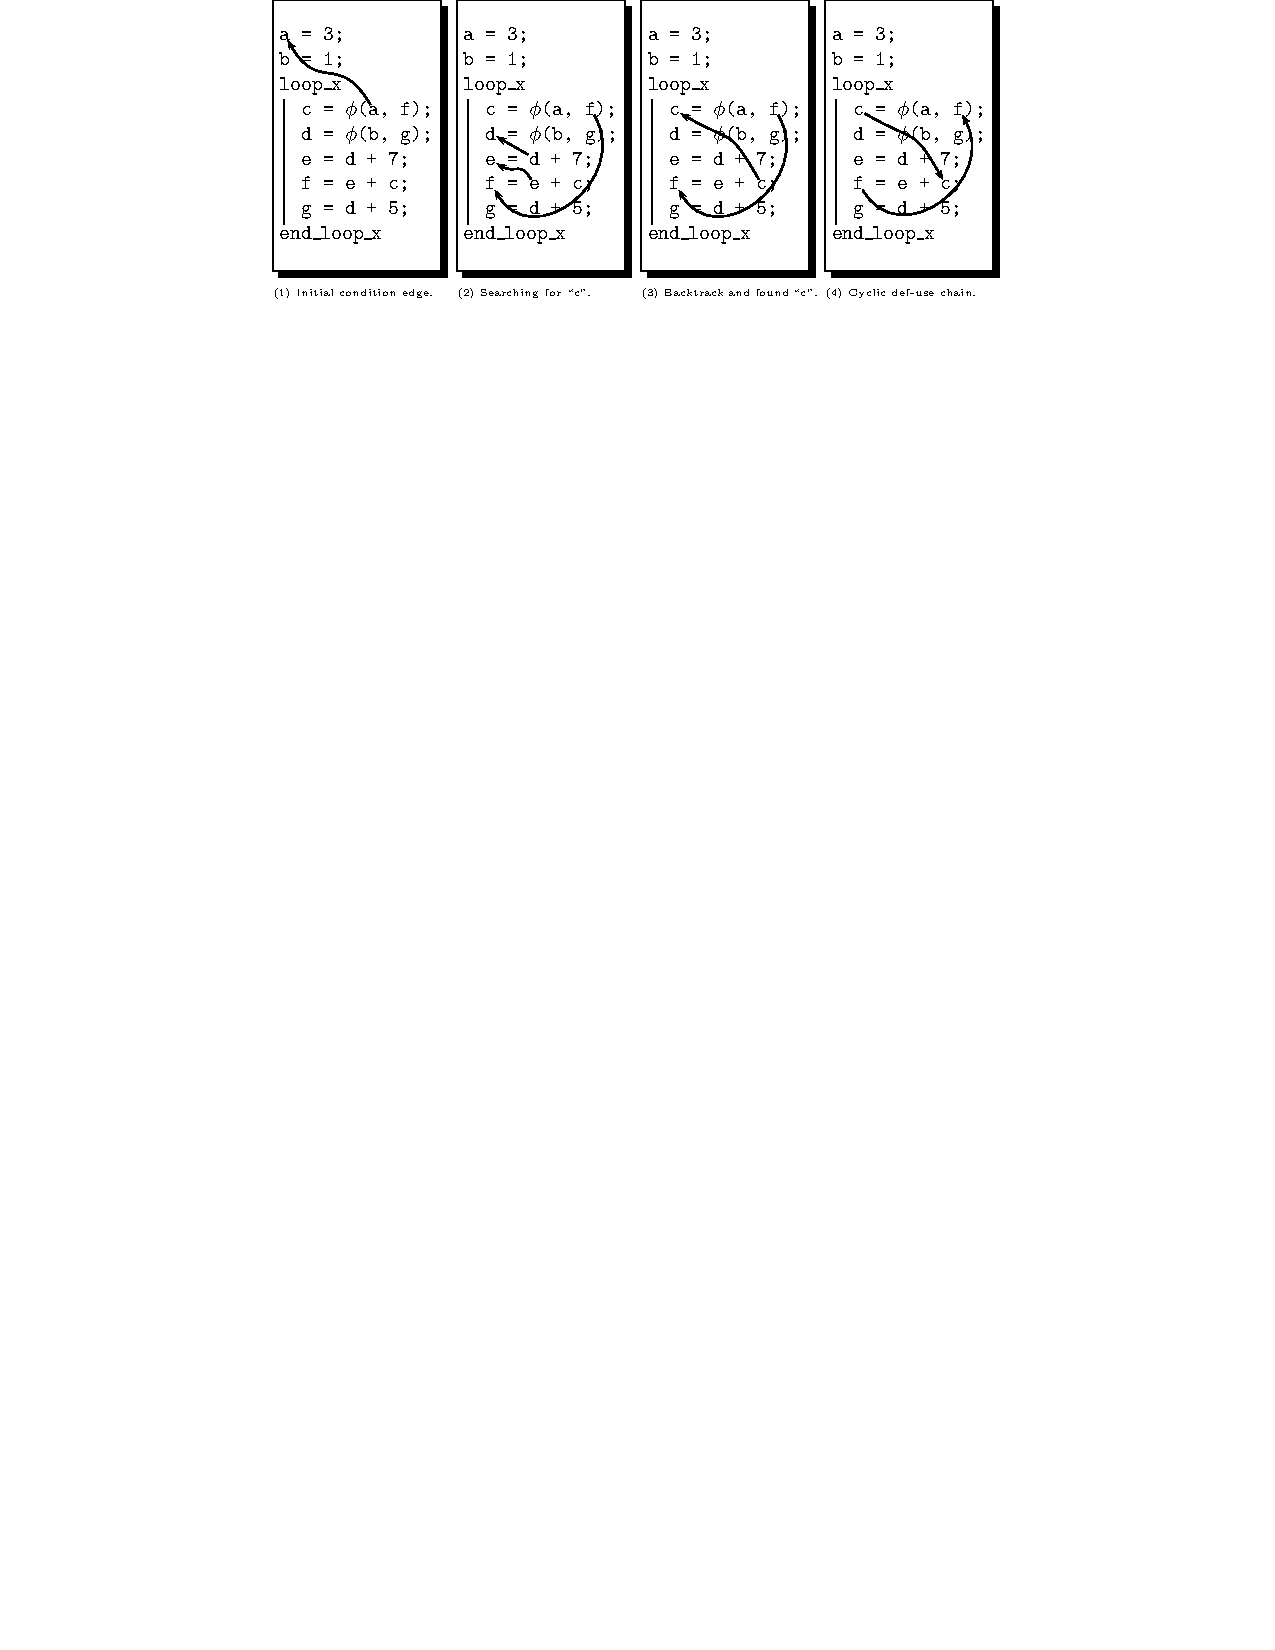
\includegraphics[width=1.2\textwidth]{fig/iv_step}
  \end{center}
  \vspace{-50em}
  \caption{Detection of the cyclic definition.}
  \label{spop:fig:ivstep}
\end{figure}

Let's look at an example, presented in Figure~\ref{spop:fig:ivstep},
to see how this algorithm works.  The arguments of a phi node are
analyzed to determine whether they contain self references or if they
are pointing towards the initial value of the induction variable.  In
this example, (1) represents the edge that points towards the
invariant definition.  When the argument to be analyzed points towards
a longer use-def chain, the full chain is traversed, as shown in (2),
until a phi node is reached.  In this example, the phi node that is
reached in (2) is different to the phi node from which the analysis
started, and so in (3) a backtrack search starts, exploring the uses
that have not yet been analyzed.  When the original phi node is found,
as in (3), the cyclic def-use chain provides the step of the induction
variable: in this example, the step is ``+ e''.  Knowing the symbolic
expression for the step of the induction variable may not be enough,
as we will see next, one has to instantiate all the symbols defined in
the varying loop to precisely characterize the induction variable.

\subsection{Translation to chains of recurrences}

Once the cyclic def-use chain has been outlined and the overall loop
update expression has been identified, it is possible to translate the
sequence of values of the induction variable to a chain of recurrence
\cite{BWZ94,KMZ98,Zim01}.  The syntax of a polynomial chain of
recurrence is: $\CHREC{base, +, step}_x$, where ``base'' and ``step''
may be arbitrary expressions or constants, and ``x'' is the loop in
which the sequence is generated.  Note that when ``base'' or ``step''
translates to sequences variating in outer loops, the resulting
sequence is represented by a multivariate chain of recurrences.  When
``step'' translates into a sequence variating in the same loop ``x'',
the chain of recurrence represents a polynomial of a higher degree.

The semantics of the chains of recurrences is defined by the equation:
\begin{equation*}
  \CHREC{c_0,+,c_1,+,c_2,+,\ldots,+,c_n}_k(\vec{\ell})=
  \sum_{p=0}^{n}c_{p}\binom{\ell_k}{p}.
\end{equation*}

This semantics allows the rewriting rule:
\begin{equation*}
  \CHREC{c_0, +, \CHREC{c_1, +, c_2}_x}_x = \CHREC{c_0, +, c_1, +, c_2}_x
\end{equation*}
that is very useful in the analysis of induction variables, as it
allows the partial analysis of the outer induction variable: first,
the step part is left in a symbolic form, and then, by instantiating
the step, the chain of recurrence is that of a higher degree
polynomial.

\subsection{Instantiation of symbols and region parameters}

The last step of the induction variable analysis consists in the
instantiation (or further analysis) of symbolic expressions left from
the first step.  This includes the analysis of induction variables in
outer loops, the analysis of the end value of a loop preceding the
analyzed loop, and the replacement of any definitions occurring in
sequence before the loop with their defined expression.  In some
cases, it becomes necessary to leave in a symbolic form every
definition outside a given region, and these symbols are then called
parameters of the region.

Let's look again at the example of Figure~\ref{spop:fig:ivstep} to
see how the sequence of values of the induction variable ``c'' is
characterized with the chains of recurrences notation.  The first
step, after the cyclic definition is detected, is the translation of
this information into a chain of recurrence: in this example, the
initial value (or base of the induction variable) is ``a'' and the
step is ``e'', and so ``c'' is represented by a chain of recurrence
$\CHREC{a, +, e}_1$ that is variating in loop number $1$.  The symbols
are then instantiated: ``a'' is trivially replaced by its definition
leading to $\CHREC{3, +, e}_1$.  The analysis of ``e'' provides this
chain of recurrence: $\CHREC{8, +, 5}_1$ that is then used in the
chain of recurrence of ``c'', $\CHREC{3, +, \CHREC{8, +, 5}_1}_1$ and
that is equivalent to $\CHREC{3, +, 8, +, 5}_1$, a polynomial of
degree two.

\subsection{Number of iterations and computation of the end of loop value}

One of the important properties of loops is their trip count (i.e.,
the number of times the loop body is executed before the exit
condition becomes true).  In simple loops, the exit condition of the
loop is a comparison of an induction variable against some constant,
parameter, or another induction variable.  The number of iterations is
then computed as the solution of an equation with integer coefficients
and integer solutions, also called a Diophantine equation.  When one
or more coefficients of the Diophantine equation are parameters, the
solution is left under a parametric form.  The number of iterations
can also be an expression variating in an outer loop, in which case,
it can be characterized using a chain of recurrence expression.

With an expression representing the number of iterations in a loop, it
becomes possible to express the evolution functions of scalar
variables variating in outer loops with strides dependent on the value
computed in an inner loop: the overall effect of a loop on a scalar
variable can be computed as an apply of the number of iterations on
the evolution function (of the scalar variable) in the varying loop.

The computation of the end of loop value can also be used for
optimization purposes, for example in the case of the constant
propagation or the value range propagation after loops.

\section{Conclusion}

As we have seen in this chapter, the \CFG{} representation is embedded
in the \SSA{} structure, and properties of the \CFG{} like the
execution order and the natural loops can be detected by only looking
at the \SSA{} definitions and uses.  The detection of natural loops is
the first step in the analysis of induction variables: after the
detection of self referent definitions, it is practical to use the
chains of recurrences to characterize the sequence of values taken by
a variable during the execution of a loop.  The number of iterations
of loops can be computed based on the characterization of induction
variables.  This paves the way to advanced loop optimizations that
need both the number of iterations and induction variable
characterizations.
